\chapter{Curvature Tensors, Conservation, and Matter}

\lectureoverview{A small closed loop turns curvature into an operational
measurement: parallel transport returns a vector changed by a linear map.
In more than two dimensions that map must remember both the plane of the
loop and the vector being transported, which leads to the Riemann tensor
and its Ricci contraction. We then turn from geometry to matter. Charge
conservation motivates four-currents, energy and momentum lead to the
stress--energy tensor, and the geodesic equation closes the chain from
matter to curvature to motion.}

\section{Curvature as a Local Transport Experiment}

Begin with the two-dimensional picture. Let a vector tangent to a surface
be transported parallel to itself around a closed curve. If the enclosed
region is flat and the loop is contractible, the vector returns unchanged.
If the region is curved, the final vector is generally rotated through an
angle \(\Delta\theta\).

The loop should be small compared with the scale on which the geometry
changes. Curvature is local: an observer need not circumnavigate the Earth
to discover that its surface is curved. With sufficiently accurate rulers,
protractors, and transport experiments, a tiny neighborhood is enough.

\begin{classroomqa}
\audiencequestion{Must the closed curves be small?
\lecturetimestamp{00:02:42--00:03:51}}
\lecturerresponse{For the local curvature measurement, yes. We shrink the
loop until its enclosed area is infinitesimal. Large loops can mix local
curvature with global topology, whereas the infinitesimal limit isolates
the geometry at the base point.}
\end{classroomqa}

Nothing in this experiment requires an embedding space. Imagine a bug
confined to the surface. Its light rays, rulers, and protractors all lie
within the surface, so it can compare lengths, angles, and transported
directions without ever looking outward. These are \emph{intrinsic}
measurements. How the surface bends in some surrounding space is
\emph{extrinsic} information and is not part of the present definition.

\begin{classroomqa}
\audiencequestion{The drawing shows a surface embedded in three
dimensions. Is the curvature being defined by that embedding?
\lecturetimestamp{00:03:53--00:06:03}}
\lecturerresponse{No. The drawing helps our limited visual intuition, but
the experiment belongs entirely to the surface. A creature confined there
can detect the curvature with tangent rulers and parallel transport. The
same intrinsic construction makes sense for a space-time that is not
presented as a hypersurface in anything larger.}
\end{classroomqa}

A rigid two-wheel cart gives a mechanical picture of intrinsic straight
motion. Equal wheels constrained not to turn relative to one another roll
straight on a plane and follow a geodesic on a curved surface. A
gyroscope gives another picture: its axis supplies a direction that can be
carried while the base point moves. Neither analogy replaces the
connection, but both make the transport experiment concrete.

Choose an orientation for the loop and for positive vector rotation. In
two dimensions the leading small-loop law is
\begin{equation}
  \Delta\theta
  =
  K(p)\,\Delta A
  +
  O\!\left((\Delta A)^{3/2}\right),
  \label{eq:l07-gaussian-holonomy}
\end{equation}
where \(K\) is Gaussian curvature and \(\Delta A\) is oriented area.
Reversing the loop reverses \(\Delta\theta\). A sphere has positive
curvature under the usual convention; a saddle has negative curvature.

\begin{figure}[tbp]
  \centering
  
\includegraphics[width=0.88\textwidth]{lecture_07_figure_01.png}
  \caption{The surface loop and the board relation
  \(d\theta/dA=R\). In these notes the two-dimensional coefficient is
  denoted by \(K\), reserving \(R\) for curvature tensors and their
  contractions.}
  \lectureframe{00:11:47}
\end{figure}

\section{Two Planes in More Than Two Dimensions}

On a surface there is only one tangent plane, so the rotation angle nearly
contains the whole story. In \(D>2\), two distinct geometric choices
appear.

First, the infinitesimal loop lies in a plane selected by two displacement
directions, say \(x^\mu\) and \(x^\nu\). Second, parallel transport acts on
the initial vector and may rotate or mix its components in another plane.
In three dimensions one may replace each oriented plane by a dual axis,
but that shortcut is special to three dimensions. In arbitrary dimension
the pair of directions must be kept explicitly.

\begin{figure}[tbp]
  \centering
  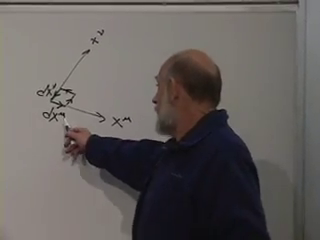
\includegraphics[width=0.86\textwidth]{lecture_07_figure_02.png}
  \caption{An infinitesimal coordinate rectangle in the
  \(x^\mu\)-\(x^\nu\) plane. Its two directed edges identify the plane and
  orientation on which the curvature map is evaluated.}
  \lectureframe{00:19:08}
\end{figure}

Transporting an orthonormal gyroscope triad illustrates the second plane.
The triad may return rotated about an axis unrelated to the axis normal to
the loop. The curvature therefore cannot be represented by one scalar in
general.

\begin{classroomqa}
\audiencequestion{Can parallel transport destroy perpendicularity between
two vectors?
\lecturetimestamp{00:16:15--00:17:30}}
\lecturerresponse{Not for the Levi--Civita connection. Metric
compatibility gives
\[
  \frac{D}{Ds}\bigl(g_{\rho\sigma}U^\rho V^\sigma\bigr)=0
\]
when both vectors are parallel transported. Lengths and mutual angles,
including a right angle, are preserved. More general affine connections
need not have this property.}
\end{classroomqa}

\section{The Infinitesimal Rectangle}

Let \(V^\rho\) be transported along a curve. Parallel transport is defined
by
\begin{equation}
  \frac{D V^\rho}{Ds}
  =
  \frac{dV^\rho}{ds}
  +
  \Gamma^\rho{}_{\sigma\mu}V^\sigma
  \frac{dx^\mu}{ds}
  =0.
  \label{eq:l07-parallel-transport}
\end{equation}
For one infinitesimal displacement this becomes
\begin{equation}
  dV^\rho
  =
  -\Gamma^\rho{}_{\sigma\mu}V^\sigma\,dx^\mu.
  \label{eq:l07-incremental-transport}
\end{equation}

\begin{figure}[tbp]
  \centering
  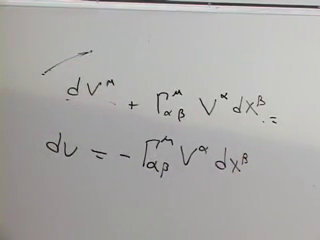
\includegraphics[width=0.89\textwidth]{lecture_07_figure_03.png}
  \caption{The board form of the infinitesimal parallel-transport law.
  The connection changes vector components as the base point moves.}
  \lectureframe{00:24:23}
\end{figure}

Now follow the four sides of a genuinely closed infinitesimal rectangle
with edge vectors \(\epsilon^\mu\) and \(\eta^\nu\). Contributions that
would occur on a path followed immediately by its reverse cancel.
Neighboring sides do not cancel completely because the connection on the
second side is evaluated at a displaced point, and because successive
connection matrices need not commute.

The surviving change is bilinear in the two edge vectors and linear in
the initial vector:
\begin{equation}
  \delta V^\rho
  =
  R^\rho{}_{\sigma\mu\nu}
  V^\sigma\epsilon^\mu\eta^\nu
  +
  O(\ell^3).
  \label{eq:l07-small-loop-map}
\end{equation}
Here \(\ell\) is a characteristic edge length. The antisymmetric
combination
\begin{equation}
  \Sigma^{\mu\nu}
  =
  \epsilon^\mu\eta^\nu-\epsilon^\nu\eta^\mu
  \label{eq:l07-area-bivector}
\end{equation}
is the oriented area bivector. It is more precise than calling the area
the simple product of two edge lengths, since the coordinate directions
need not be orthogonal or normalized.

\begin{figure}[tbp]
  \centering
  
\includegraphics[width=0.88\textwidth]{lecture_07_figure_04.png}
  \caption{The board separates the two displacement directions, the
  transported vector component, and the four-index curvature coefficient.
  Together they form the linear holonomy map in
  Eq.~\eqref{eq:l07-small-loop-map}.}
  \lectureframe{00:27:53}
\end{figure}

\begin{classroomqa}
\audiencequestion{One index was used twice for different roles. Which
indices belong to the vector, and which belong to the loop?
\lecturetimestamp{00:20:57--00:21:10}}
\lecturerresponse{Use four distinct slots. In
\(R^\rho{}_{\sigma\mu\nu}\), the index \(\sigma\) selects the initial
component of \(V\), \(\rho\) selects the resulting component, and
\(\mu,\nu\) identify the oriented loop plane. Repeated indices are summed
only after those roles have been separated.}
\end{classroomqa}

\begin{classroomqa}
\audiencequestion{Are the two infinitesimal displacements the same
quantity, and are their indices summed?
\lecturetimestamp{00:36:31--00:37:40}}
\lecturerresponse{They are the two independently chosen edge vectors of
the small loop. Their components contract with the last two curvature
indices. Writing \(\epsilon^\mu\eta^\nu\), or equivalently the area
bivector \(\Sigma^{\mu\nu}\), prevents the two directions from being
mistaken for one displacement.}
\end{classroomqa}

\section{The Riemann Curvature Tensor}

We fix the convention
\begin{equation}
  [\nabla_\mu,\nabla_\nu]V^\rho
  =
  R^\rho{}_{\sigma\mu\nu}V^\sigma.
  \label{eq:l07-riemann-convention}
\end{equation}
With this convention,
\begin{align}
  R^\rho{}_{\sigma\mu\nu}
  &=
  \partial_\mu\Gamma^\rho{}_{\nu\sigma}
  -
  \partial_\nu\Gamma^\rho{}_{\mu\sigma}
  \nonumber\\
  &\quad
  +
  \Gamma^\rho{}_{\mu\lambda}
  \Gamma^\lambda{}_{\nu\sigma}
  -
  \Gamma^\rho{}_{\nu\lambda}
  \Gamma^\lambda{}_{\mu\sigma}.
  \label{eq:l07-riemann-components}
\end{align}
Changing the order in the commutator or reversing the loop orientation
changes the overall sign. Once a convention is declared, every later
formula must follow it consistently.

\begin{figure}[tbp]
  \centering
  
\includegraphics[width=0.93\textwidth]{lecture_07_figure_05.png}
  \caption{The camera follows the completed Riemann expression across the
  board; this frame records its derivative and ordered quadratic terms.
  Equation~\eqref{eq:l07-riemann-components} reconstructs the full line.}
  \lectureframe{00:32:23}
\end{figure}

Although individual Christoffel symbols are not tensor components, the
combination in Eq.~\eqref{eq:l07-riemann-components} is tensorial. The
geometric reason is more illuminating than a long transformation-law
calculation. Transport around the loop starts and ends at the same point,
so \(\delta V^\rho\) is the difference of two vectors in one tangent
space. Equation~\eqref{eq:l07-small-loop-map} holds for every initial
vector and every oriented infinitesimal area. Its multilinear coefficient
must therefore transform as a tensor.

\begin{classroomqa}
\audiencequestion{Why is the curvature coefficient a tensor when it is
built from non-tensorial Christoffel symbols?
\lecturetimestamp{00:32:42--00:34:44}}
\lecturerresponse{The non-tensorial pieces cancel in precisely the
combination above. Operationally, the closed-loop change is a vector at
the original point, and it depends linearly on the initial vector and the
two edge vectors. That coordinate-independent multilinear map is the
Riemann tensor.}
\end{classroomqa}

For each fixed direction \(\mu\), regard
\((\Gamma_\mu)^\rho{}_\sigma=\Gamma^\rho{}_{\mu\sigma}\) as a matrix.
Then the quadratic terms are a matrix commutator:
\begin{equation}
  R_{\mu\nu}
  =
  \partial_\mu\Gamma_\nu
  -
  \partial_\nu\Gamma_\mu
  +
  [\Gamma_\mu,\Gamma_\nu].
  \label{eq:l07-matrix-curvature}
\end{equation}
Because matrix multiplication is not generally commutative, the two
orders give distinct terms.

\begin{figure}[tbp]
  \centering
  
\includegraphics[width=0.91\textwidth]{lecture_07_figure_06.png}
  \caption{The two quadratic connection products are highlighted in
  opposite order. Their difference is the commutator term in the
  curvature.}
  \lectureframe{00:36:08}
\end{figure}

\begin{classroomqa}
\audiencequestion{Are the quadratic terms literally a commutator?
\lecturetimestamp{00:34:44--00:36:31}}
\lecturerresponse{Yes. Once the first and last tensor slots are treated
as matrix indices, the products are
\(\Gamma_\mu\Gamma_\nu-\Gamma_\nu\Gamma_\mu\). Together with the
derivative terms they form the commutator of covariant derivatives in
Eq.~\eqref{eq:l07-riemann-convention}.}
\end{classroomqa}

\subsection{Normal coordinates do not remove curvature}

At any regular point \(p\), normal coordinates can be chosen so that
\begin{equation}
  g_{\mu\nu}(p)=\eta_{\mu\nu},
  \qquad
  \partial_\lambda g_{\mu\nu}(p)=0,
  \qquad
  \Gamma^\rho{}_{\mu\nu}(p)=0.
  \label{eq:l07-normal-coordinates}
\end{equation}
The second derivatives of the metric do \emph{not} generally vanish.
They contain the first locally invariant information about curvature.
At \(p\), Eq.~\eqref{eq:l07-riemann-components} loses its quadratic
connection terms, but derivatives of the connection remain. This is why
gravity can be removed at one event while tidal effects cannot.

\begin{classroomqa}
\audiencequestion{How would an observer actually keep a vector parallel
while moving over a curved Earth?
\lecturetimestamp{00:37:49--00:42:49}}
\lecturerresponse{One may carry a gyroscope, or repeatedly compare the
vector with a locally inertial orthonormal frame. In coordinates the same
instruction is \(DV^\rho/Ds=0\). A tangent transported along a geodesic
continues straight; other vectors are transported by the same connection.
Normal coordinates simplify the rule at one point, not along the whole
route.}
\end{classroomqa}

\section{Symmetries and Independent Components}

Lower the first index with the metric:
\begin{equation}
  R_{\alpha\beta\mu\nu}
  =
  g_{\alpha\rho}R^\rho{}_{\beta\mu\nu}.
  \label{eq:l07-lowered-riemann}
\end{equation}

\begin{figure}[tbp]
  \centering
  
\includegraphics[width=0.90\textwidth]{lecture_07_figure_07.png}
  \caption{Lowering the output index produces the fully covariant Riemann
  tensor, the form in which its pair symmetries are easiest to state.}
  \lectureframe{00:44:08}
\end{figure}

For the torsion-free Levi--Civita connection,
\begin{align}
  R_{\alpha\beta\mu\nu}
  &=-R_{\beta\alpha\mu\nu},
  \label{eq:l07-first-antisymmetry}\\
  R_{\alpha\beta\mu\nu}
  &=-R_{\alpha\beta\nu\mu},
  \label{eq:l07-second-antisymmetry}\\
  R_{\alpha\beta\mu\nu}
  &=R_{\mu\nu\alpha\beta},
  \label{eq:l07-pair-exchange}\\
  R_{\alpha[\beta\mu\nu]}
  &=0.
  \label{eq:l07-bianchi}
\end{align}
The last line is the first Bianchi identity. The tensor is antisymmetric
within each index pair, symmetric under exchange of the pairs, and
subject to one cyclic identity. It is not assigned a sign by an arbitrary
permutation of all four indices.

\begin{figure}[tbp]
  \centering
  
\includegraphics[width=0.93\textwidth]{lecture_07_figure_08.png}
  \caption{The board develops antisymmetry within an index pair. The
  completed relations are Eqs.~\eqref{eq:l07-first-antisymmetry}--%
  \eqref{eq:l07-bianchi}.}
  \lectureframe{00:47:48}
\end{figure}

\begin{classroomqa}
\audiencequestion{Does reversing the loop reverse the transport effect?
\lecturetimestamp{00:44:52--00:45:20}}
\lecturerresponse{Yes. Reversing the oriented area exchanges
\(\mu\) and \(\nu\), and
\(R^\rho{}_{\sigma\mu\nu}=-R^\rho{}_{\sigma\nu\mu}\).
The leading holonomy therefore changes sign.}
\end{classroomqa}

\begin{classroomqa}
\audiencequestion{Can every permutation be handled by attaching the sign
of the permutation, and how many independent components remain?
\lecturetimestamp{00:48:38--00:52:52}}
\lecturerresponse{No. Only the stated pair operations have simple signs,
and the Bianchi identity supplies an additional relation. In \(D\)
dimensions the number of independent components is
\[
  N_R=\frac{D^2(D^2-1)}{12}.
\]
Thus \(N_R=1\) in two dimensions, \(6\) in three dimensions, and \(20\)
in four dimensions. The tentative board count is corrected by including
all pair symmetries and the cyclic identity.}
\end{classroomqa}

For a two-sphere of radius \(a\),
\begin{equation}
  K=\frac{1}{a^2}.
  \label{eq:l07-sphere-curvature}
\end{equation}
The unique independent curvature component in two dimensions is
therefore fixed by one scalar function.

\begin{classroomqa}
\audiencequestion{How does the sphere's radius enter the curvature?
\lecturetimestamp{00:54:12--00:54:57}}
\lecturerresponse{The Gaussian curvature is \(1/a^2\). A larger sphere
looks flatter on a fixed small patch, and the same small area produces a
smaller holonomy angle.}
\end{classroomqa}

The infinitesimal path must actually close. A coordinate parallelogram is
only a convenient leading-order construction. For the torsion-free
connection used here, one may choose a genuinely closed small loop whose
shape corrections change only higher-order terms; the leading
area-curvature relation remains Eq.~\eqref{eq:l07-small-loop-map}.

\begin{classroomqa}
\audiencequestion{What if the four prescribed displacements fail to close
exactly?
\lecturetimestamp{00:55:01--00:57:40}}
\lecturerresponse{Define a closed parameterized loop first, then expand
its holonomy. In a torsion-free geometry the small coordinate rectangle
can be corrected at higher order without changing the leading
\(R\cdot\Sigma\) term. An open path would compare vectors at different
points and would not by itself define the same local curvature
measurement.}
\end{classroomqa}

\begin{figure}[tbp]
  \centering
  
\includegraphics[width=0.88\textwidth]{lecture_07_figure_09.png}
  \caption{The board returns to the small-loop relation: the curvature
  tensor contracts with two directed edge elements and the transported
  vector to give the leading vector change.}
  \lectureframe{00:53:23}
\end{figure}

\section{The Ricci Contraction}

One contraction of the Riemann tensor is especially important:
\begin{equation}
  R_{\beta\nu}
  =
  R^\alpha{}_{\beta\alpha\nu}
  =
  g^{\alpha\mu}R_{\alpha\beta\mu\nu}.
  \label{eq:l07-ricci}
\end{equation}
For the Levi--Civita connection, the Ricci tensor is symmetric:
\begin{equation}
  R_{\beta\nu}=R_{\nu\beta}.
  \label{eq:l07-ricci-symmetric}
\end{equation}
Contracting once more gives the Ricci scalar,
\begin{equation}
  R=g^{\beta\nu}R_{\beta\nu}.
  \label{eq:l07-ricci-scalar}
\end{equation}

\begin{figure}[tbp]
  \centering
  
\includegraphics[width=0.91\textwidth]{lecture_07_figure_10.png}
  \caption{The Ricci tensor is obtained by contracting one index from
  each antisymmetric pair of the Riemann tensor.}
  \lectureframe{01:02:23}
\end{figure}

In three dimensions the Riemann tensor contains no information beyond the
Ricci tensor. Explicitly,
\begin{align}
  R_{abcd}
  &=
  g_{ac}R_{bd}-g_{ad}R_{bc}
  -g_{bc}R_{ad}+g_{bd}R_{ac}
  \nonumber\\
  &\quad
  -\frac{R}{2}
  \left(g_{ac}g_{bd}-g_{ad}g_{bc}\right).
  \label{eq:l07-three-dimensional-riemann}
\end{align}
In four dimensions this is no longer true; the Weyl tensor carries the
remaining curvature information.

\begin{classroomqa}
\audiencequestion{What geometric problem does the Ricci tensor solve?
\lecturetimestamp{01:03:31--01:05:27}}
\lecturerresponse{It is the natural trace of the full curvature map. In
three dimensions it determines all of the Riemann tensor, as
Eq.~\eqref{eq:l07-three-dimensional-riemann} shows. In four-dimensional
space-time it does not determine every tidal degree of freedom, but it is
the contraction that enters the Einstein tensor and hence the field
equation.}
\end{classroomqa}

\section{From Geometry to Matter}

We have reached the geometric half of general relativity. Curvature is the
coordinate-independent obstruction measured by small-loop transport and,
physically, by tidal relative acceleration. The other half asks what
produces that curvature.

The answer cannot be mass density alone. Special relativity mixes energy
and momentum between frames, so a relativistic source must contain local
densities and fluxes of both. Before constructing it, we use electric
charge as a simpler conserved quantity.

\section{Charge Density and Current}

For a small spatial volume \(\Delta V\) containing charge \(\Delta Q\),
define
\begin{equation}
  \rho_q
  =
  \lim_{\Delta V\to0}\frac{\Delta Q}{\Delta V}.
  \label{eq:l07-charge-density}
\end{equation}
The charge in a region \(\Omega\) is
\begin{equation}
  Q_\Omega(t)
  =
  \int_\Omega \rho_q(t,\mathbf x)\,d^3x.
  \label{eq:l07-total-charge}
\end{equation}

\begin{figure}[tbp]
  \centering
  
\includegraphics[width=0.86\textwidth]{lecture_07_figure_11.png}
  \caption{A small volume element and the local definition
  \(\rho_q=dQ/dV\). Charge itself is not a space-time component; its
  density depends on the spatial slice.}
  \lectureframe{01:09:23}
\end{figure}

Imagine the fixed spatial region extended through time. It becomes a
world-tube. Charged particles trace worldlines through that tube. Charge
inside the spatial box may change because worldlines cross its side
boundary, even though the total charge of the complete isolated system is
constant. Under local conservation, charge worldlines do not simply end
at one event and begin at an unrelated distant event.

\begin{figure}[tbp]
  \centering
  
\includegraphics[width=0.88\textwidth]{lecture_07_figure_12.png}
  \caption{A spatial box extended in time. Charge worldlines cross the
  boundary, turning change of enclosed charge into a flux statement.}
  \lectureframe{01:11:53}
\end{figure}

The current component \(j^i\) measures charge crossing an oriented area
normal to the \(i\)-direction per unit area per unit time:
\begin{equation}
  j^i
  =
  \frac{dQ}{dA_i\,dt}.
  \label{eq:l07-current-density}
\end{equation}
When \(c=1\), time and distance have the same units, so charge density and
current density fit naturally into one four-vector,
\begin{equation}
  J^\mu=(\rho_q,j^1,j^2,j^3).
  \label{eq:l07-four-current}
\end{equation}

\begin{figure}[tbp]
  \centering
  
\includegraphics[width=0.88\textwidth]{lecture_07_figure_13.png}
  \caption{The board definitions of charge density and current through an
  oriented window, accompanied by the flux picture.}
  \lectureframe{01:17:08}
\end{figure}

\begin{figure}[tbp]
  \centering
  
\includegraphics[width=0.87\textwidth]{lecture_07_figure_14.png}
  \caption{The four-current components
  \(J^\mu=(\rho_q,j^1,j^2,j^3)\). A Lorentz transformation mixes density
  and spatial current.}
  \lectureframe{01:17:53}
\end{figure}

\section{Local Conservation}

Global conservation says that the total charge of an isolated system does
not change. Local conservation says more: charge in a region changes only
because current flows through its boundary. Without locality, charge
could disappear here and reappear far away while preserving only the
global total.

For a fixed volume \(\Omega\),
\begin{equation}
  \frac{d}{dt}\int_\Omega\rho_q\,d^3x
  =
  -\oint_{\partial\Omega}\mathbf j\cdot d\mathbf A.
  \label{eq:l07-integral-continuity}
\end{equation}
The divergence theorem gives the differential continuity equation,
\begin{equation}
  \boxed{
  \frac{\partial\rho_q}{\partial t}
  +
  \boldsymbol{\nabla}\cdot\mathbf j
  =0
  }.
  \label{eq:l07-continuity}
\end{equation}
In space-time notation,
\begin{equation}
  \partial_\mu J^\mu=0.
  \label{eq:l07-four-current-conservation}
\end{equation}

\begin{figure}[tbp]
  \centering
  
\includegraphics[width=0.93\textwidth]{lecture_07_figure_15.png}
  \caption{The continuity equation in three-dimensional and four-vector
  form. A uniform current through a box has equal inflow and outflow, so
  the enclosed density remains unchanged.}
  \lectureframe{01:24:38}
\end{figure}

\subsection{Charge is a scalar; density is not}

The total electric charge \(Q\) is Lorentz invariant. The density
\(\rho_q\) is not a scalar: changing frames changes both the spatial
volume used to define the density and the motion of the charges. What one
observer calls mostly density another may describe as a mixture of
density and current. The four-vector \(J^\mu\), not \(\rho_q\) alone, is
the covariant object.

\begin{classroomqa}
\audiencequestion{Is one coulomb of charge necessarily an enormous
explosive amount, and what does a one-farad capacitor contain?
\lecturetimestamp{01:26:12--01:31:02}}
\lecturerresponse{A capacitor stores separated charges \(+Q\) and
\(-Q\), so its net charge is zero. The exact relations are
\[
  Q=CV,
  \qquad
  U=\frac12CV^2=\frac{Q^2}{2C}.
\]
A one-farad capacitor at one volt carries one coulomb in magnitude on
each plate and stores \(0.5\) joule. That is not an explosion. By
contrast, concentrating an uncompensated net charge of one coulomb in a
small isolated object would require extreme electrostatic conditions.
The geometry and voltage matter; the unit of charge alone does not fix
the stored energy.}
\end{classroomqa}

\section{Energy and Momentum}

Energy and momentum are also conserved, but neither is separately
frame-independent. They form the four-momentum
\begin{equation}
  P^\mu=(E,p^1,p^2,p^3)
  \qquad(c=1).
  \label{eq:l07-four-momentum}
\end{equation}
A body at rest in one frame has energy and no spatial momentum; a moving
observer assigns it both kinetic energy and momentum. Consequently, local
energy conservation and the three local momentum-conservation laws must
be components of one covariant statement.

\begin{figure}[tbp]
  \centering
  
\includegraphics[width=0.86\textwidth]{lecture_07_figure_16.png}
  \caption{Energy and three-momentum assembled into the four-momentum
  \(P^\mu\). Lorentz transformations mix its components.}
  \lectureframe{01:33:23}
\end{figure}

\section{The Stress--Energy Tensor}

The local relativistic source is the stress--energy tensor
\(T^{\nu\mu}\). We use the lecture's bookkeeping convention: the first
index \(\nu\) labels the conserved quantity and the second index \(\mu\)
labels the direction of flux. Then
\begin{align}
  T^{00}
  &=
  \text{energy density},
  \label{eq:l07-t00}\\
  T^{0i}
  &=
  \text{flux of energy in direction \(i\)},
  \label{eq:l07-t0i}\\
  T^{i0}
  &=
  \text{density of \(i\)-momentum},
  \label{eq:l07-ti0}\\
  T^{ij}
  &=
  \text{flux of \(i\)-momentum across a surface normal to \(j\)}.
  \label{eq:l07-tij}
\end{align}
The spatial block \(T^{ij}\) is the stress tensor. Its diagonal entries
are pressures or normal stresses; its off-diagonal entries are shear
stresses. A stream of particles moving obliquely, for example, can carry
\(x\)-momentum across a surface whose normal points in the \(y\)-direction.

\begin{equation}
  T^{\mu\nu}
  =
  \begin{pmatrix}
    T^{00} & T^{01} & T^{02} & T^{03}\\
    T^{10} & T^{11} & T^{12} & T^{13}\\
    T^{20} & T^{21} & T^{22} & T^{23}\\
    T^{30} & T^{31} & T^{32} & T^{33}
  \end{pmatrix}.
  \label{eq:l07-stress-energy-matrix}
\end{equation}

\begin{figure}[tbp]
  \centering
  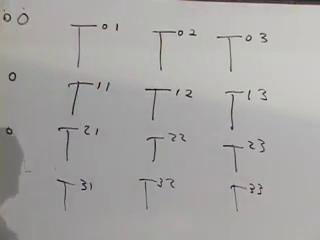
\includegraphics[width=0.88\textwidth]{lecture_07_figure_17.png}
  \caption{The complete \(4\times4\) array of stress--energy components.
  Rows label energy or a momentum component; columns distinguish density
  from the three flux directions.}
  \lectureframe{01:41:23}
\end{figure}

For the standard symmetric stress--energy tensor used as the
gravitational source,
\begin{equation}
  T^{\mu\nu}=T^{\nu\mu}.
  \label{eq:l07-stress-energy-symmetric}
\end{equation}
Microscopically, energy flux equals momentum density in units \(c=1\).
For fields with intrinsic spin, the canonical tensor can first be
nonsymmetric; the symmetric, conserved tensor coupled to gravity is
obtained by the standard improvement.

\begin{classroomqa}
\audiencequestion{Is the array automatically a tensor merely because its
entries describe physical quantities?
\lecturetimestamp{01:42:23--01:43:00}}
\lecturerresponse{Physical meaning motivates the construction but does
not by itself prove a transformation law. One proves tensoriality by a
covariant microscopic or field-theoretic definition, or by showing how
the local density and fluxes transform under Lorentz changes of frame.
Once that is done, the component interpretations above follow in every
local inertial frame.}
\end{classroomqa}

\section{Four Local Conservation Laws}

Each row obeys a continuity equation. With the index convention just
chosen,
\begin{equation}
  \frac{\partial T^{\nu0}}{\partial t}
  +
  \frac{\partial T^{\nu1}}{\partial x}
  +
  \frac{\partial T^{\nu2}}{\partial y}
  +
  \frac{\partial T^{\nu3}}{\partial z}
  =0.
  \label{eq:l07-stress-energy-continuity}
\end{equation}
Equivalently,
\begin{equation}
  \boxed{
  \partial_\mu T^{\nu\mu}=0
  }.
  \label{eq:l07-flat-stress-conservation}
\end{equation}
If the symmetric convention \(T^{\mu\nu}=T^{\nu\mu}\) is already in use,
this is the familiar \(\partial_\mu T^{\mu\nu}=0\).

\begin{figure}[tbp]
  \centering
  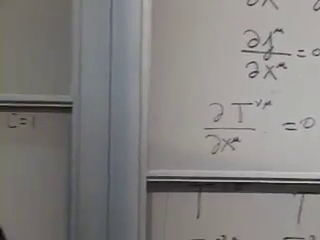
\includegraphics[width=0.88\textwidth]{lecture_07_figure_18.png}
  \caption{The four compact conservation equations for energy and
  momentum, written as the divergence of \(T^{\nu\mu}\).}
  \lectureframe{01:46:08}
\end{figure}

Equation~\eqref{eq:l07-flat-stress-conservation} is written with ordinary
derivatives because we have described a local inertial frame in special
relativity. In curved space-time the covariant statement is
\begin{equation}
  \nabla_\mu T^{\nu\mu}=0.
  \label{eq:l07-covariant-stress-conservation}
\end{equation}

\begin{classroomqa}
\audiencequestion{Why are ordinary derivatives being used if the goal is
general relativity?
\lecturetimestamp{01:46:31--01:46:54}}
\lecturerresponse{The matter tensor is first organized in a local
inertial frame, where the connection vanishes at the chosen event. The
curved-space equation is obtained by replacing the ordinary divergence
with the covariant divergence.}
\end{classroomqa}

\section{Curvature, Sources, and Geodesic Motion}

The structure of general relativity is now visible even before the field
equation is written:
\begin{equation}
  T_{\mu\nu}
  \longrightarrow
  \text{space-time curvature}
  \longrightarrow
  \text{geodesic motion}.
  \label{eq:l07-gr-chain}
\end{equation}
Mass contributes because \(E=mc^2\), but energy density is only one
component of the source. Momentum density, energy flux, pressure, and
shear must also contribute, because Lorentz transformations mix them.

A freely falling particle follows a space-time geodesic. With proper time
\(\tau\) as an affine parameter,
\begin{equation}
  \boxed{
  \frac{d^2x^\mu}{d\tau^2}
  +
  \Gamma^\mu{}_{\nu\sigma}
  \frac{dx^\nu}{d\tau}
  \frac{dx^\sigma}{d\tau}
  =0
  }.
  \label{eq:l07-geodesic}
\end{equation}

\begin{figure}[tbp]
  \centering
  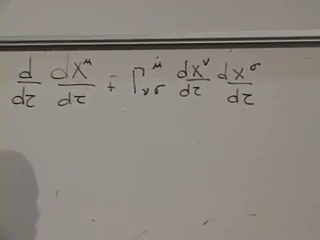
\includegraphics[width=0.92\textwidth]{lecture_07_figure_19.png}
  \caption{The completed geodesic equation. The connection turns the
  locally straight worldline into coordinate acceleration in a general
  chart.}
  \lectureframe{01:52:23}
\end{figure}

Take the slow-motion, weak-field limit. The spatial components of
\(dx^\mu/d\tau\) are small compared with the time component, and
\begin{equation}
  \frac{dt}{d\tau}\simeq1.
  \label{eq:l07-slow-time-component}
\end{equation}
For a spatial index \(i\), the dominant term in the geodesic equation is
\begin{equation}
  \frac{d^2x^i}{dt^2}
  \simeq
  -\Gamma^i{}_{00}.
  \label{eq:l07-newtonian-geodesic-limit}
\end{equation}

\begin{classroomqa}
\audiencequestion{Which component of the four-velocity remains large in
the nonrelativistic limit?
\lecturetimestamp{01:53:42--01:53:51}}
\lecturerresponse{The time component. With \(c=1\),
\(dx^0/d\tau=dt/d\tau\simeq1\), while the three spatial components are
the small ordinary velocities. That is why the \(00\) connection
coefficient dominates the spatial geodesic equation.}
\end{classroomqa}

\begin{figure}[tbp]
  \centering
  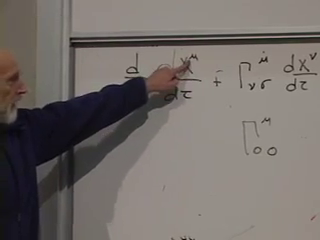
\includegraphics[width=0.91\textwidth]{lecture_07_figure_20.png}
  \caption{The geodesic equation beside the dominant weak-field
  coefficient \(\Gamma^\mu{}_{00}\). For spatial motion the acceleration
  is \(-\Gamma^i{}_{00}\) in the stated convention.}
  \lectureframe{01:55:38}
\end{figure}

For the weak static metric with signature \((+---)\),
\begin{equation}
  g_{00}\simeq1+2\Phi,
  \qquad
  \Gamma^i{}_{00}\simeq\partial_i\Phi,
  \label{eq:l07-newtonian-potential}
\end{equation}
so Eq.~\eqref{eq:l07-newtonian-geodesic-limit} becomes
\begin{equation}
  \frac{d^2\mathbf x}{dt^2}
  \simeq
  -\boldsymbol{\nabla}\Phi.
  \label{eq:l07-newtonian-acceleration}
\end{equation}
The next step is to determine how \(T_{\mu\nu}\) fixes the curvature and
hence the connection. The present lecture has assembled all the pieces
that equation must respect: tensorial curvature, local conservation, and
geodesic motion.
